\documentclass[5p,sort&compress]{elsarticle}

\usepackage{amssymb}    % Mathematical symbols
\usepackage{amsmath}    % More options for mathematics
\usepackage{subfigure}  % More options for figures
\usepackage{epstopdf}   % Convert eps to pdf
\usepackage[separate-uncertainty=true]{siunitx}   % Proper formatting of units in math mode
\usepackage{color}      % Supports text color if needed
\usepackage{soul}       % https://ctan.org/pkg/soul
\usepackage{lmodern}    % Loading fonts
\usepackage{hyperref}   % To insert clickable references/urls
\usepackage{listings}   % To input code in the text
\usepackage{amsmath}
\usepackage{amsmath}
\usepackage{amssymb}
\usepackage{graphicx}
\usepackage{epstopdf}
\usepackage{booktabs}
\setlength{\parskip}{2em}
\newcommand{\stirlingii}{\genfrac{\{}{\}}{0pt}{}}

% Choose the style of the reference list (do not change)
\bibliographystyle{elsarticle-num}

\journal{ifding/learning-notes}

% Begin the document

\begin{document}

\begin{frontmatter}
    \title{Ch 5: Neural Networks}
    \author{ifding}
    
    \begin{abstract}
        Feed-forward Network, Network Training, Mixture Density Networks, Bayesian Neural Networks
    \end{abstract}


\end{frontmatter}

%% How to make a heading and divide the documents into different sections

\section{Feed-forward Network}

First we construct M linear combinations of the input variables $x_1, \ldots, x_D$ in the form
\begin{equation}
a_{j}=\sum_{i=1}^{D} w_{j i}^{(1)} x_{i}+w_{j 0}^{(1)}
\end{equation}
where $j=1,\ldots, M$, and the superscript (1) indicates that the corresponding parameters are in the first `layer' of the network. Each of them is transformed using a differentiable, nonlinear \textit{activation function} $h(\cdot)$ to give
\begin{equation}
z_j = h(a_j)
\end{equation}
\begin{equation}
a_{k}=\sum_{j=1}^{M} w_{k j}^{(2)} z_{j}+w_{k 0}^{(2)}
\end{equation}
where $k=1, \ldots, K$, and K is the total number of outputs.

\begin{figure}[ht]
     \centering
     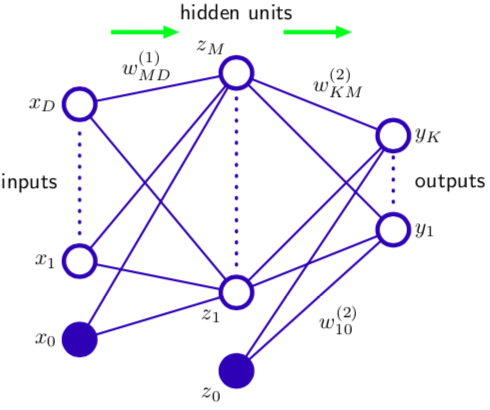
\includegraphics[width = \linewidth]{figure/figure5_1.png}
     \caption{Two-layer neural network.}
     \label{fig:nn}
\end{figure}

As shown in Figure~\ref{fig:nn}, for binary classification problems, 
\begin{equation}
    y_k = \sigma(a_k)
\end{equation}
where 
\begin{equation}
\sigma(a)=\frac{1}{1+\exp (-a)}
\end{equation}

We can absorb the biases into the layers' weights,so
\begin{equation}
y_{k}(\mathbf{x}, \mathbf{w})=\sigma\left(\sum_{j=0}^{M} w_{k j}^{(2)} h\left(\sum_{i=0}^{D} w_{j i}^{(1)} x_{i}\right)\right)
\end{equation}


\section{Network Training}

A simple approach to the problem of determining the network parameters is to minimize a sum-of-squares error function. 
Given a data set of N independent, identically distributed observations $\mathbf{X} = \{\mathbf{x}_1, \ldots, \mathbf{x}_n\}$ and target vectors $\mathbf{t} = \{\mathbf{t}_n\}$, where $n = 1, \ldots, N$, we can construct the corresponding likelihood function
\begin{equation}
p(\mathbf{t} | \mathbf{X}, \mathbf{w}, \beta)=\prod_{n=1}^{N} p\left(t_{n} | \mathbf{x}_{n}, \mathbf{w}, \beta\right)
\end{equation}
Taking the negative logarithm, we obtain the error function
\begin{equation}
\frac{\beta}{2} \sum_{n=1}^{N}\left\{y\left(\mathbf{x}_{n}, \mathbf{w}\right)-t_{n}\right\}^{2}-\frac{N}{2} \ln \beta+\frac{N}{2} \ln (2 \pi)
\end{equation}
Maximizing the likelihood function is equivalent to minimizing the sum-of-squares error function given by
\begin{equation}
E(\mathbf{w})=\frac{1}{2} \sum_{n=1}^{N}\left\{y\left(\mathbf{x}_{n}, \mathbf{w}\right)-t_{n}\right\}^{2}
\end{equation}
where we have discarded additive and multiplicative constants. In practice, the nonlinearity of the network function $y(\mathbf{x}_n, \mathbf{w})$ causes the error $E(\mathbf{w})$ to be nonconvex.

The conditional distribution of targets given inputs is then a Bernoulli distribution of the form
\begin{equation}
p(t | \mathbf{x}, \mathbf{w})=y(\mathbf{x}, \mathbf{w})^{t}\{1-y(\mathbf{x}, \mathbf{w})\}^{1-t}
\end{equation}
The error function, which is given by the negative log likelihood, is then a \textit{cross-entropy} error function
of the form
\begin{equation}
E(\mathbf{w})=-\sum_{n=1}^{N}\left\{t_{n} \ln y_{n}+\left(1-t_{n}\right) \ln \left(1-y_{n}\right)\right\}
\end{equation}
where $y_n$ denotes $y(\mathbf{x}_n, \mathbf{w})$.

Because the error $E(\mathbf{w})$ is a smooth continuous function of w, its smallest value will occur at a point in weight space such that the gradient of the error function vanishes, so that
\begin{equation}
\nabla E(\mathbf{w})=0
\end{equation}
as otherwise we could make a small step in the direction of $-\nabla E(\mathbf{w})$ and thereby further reduce the error.

The simplest approach to using gradient information is to choose the weight update to comprise a small step in the direction of the negative gradient, so
that
\begin{equation}
\mathbf{w}^{(\tau+1)}=\mathbf{w}^{(\tau)}-\eta \nabla E\left(\mathbf{w}^{(\tau)}\right)
\end{equation}
where the parameter $\tau > 0$ is known as the \textit{learning rate}.


\section{Mixture Density Networks}

The goal of supervised learning is to model a conditional distribution $p(\mathbf{t}|x)$, which for many simple regression problems is chosen to be Gaussisan, However, practical machine learning problems can often have significantly non-Gaussian distributions.

\textit{mixture density network}, for any given value of $\mathbf{x}$, the mixture model provides a general formalism for modelling an arbitrary conditional density function $p(\mathbf{t}|\mathbf{x})$.
\begin{equation}
p(\mathbf{t} | \mathbf{x})=\sum_{k=1}^{K} \pi_{k}(\mathbf{x}) \mathcal{N}\left(\mathbf{t} | \boldsymbol{\mu}_{k}(\mathbf{x}), \sigma_{k}^{2}(\mathbf{x})\right)
\end{equation}

We now take the various parameters of the mixture model, namely the mixing coefficients $\pi(\mathbf{x})$, the means $\boldsymbol{\mu}_k (\mathbf{x})$, and the variances $\sigma_k^2(\mathbf{x})$, to be governed by the outputs of a conventional neural network that takes $\mathbf{x}$ as its input.

\begin{figure}[ht]
     \centering
     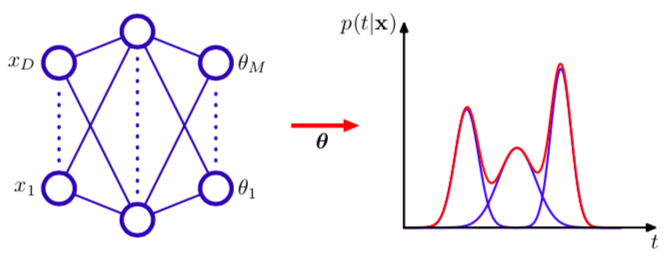
\includegraphics[width = \linewidth]{figure/figure5_20.png}
     \caption{The mixture density network}
     \label{fig:mix}
\end{figure}

The neural network in Figure~\ref{fig:mix} can, for example, be a two-layer network having sigmoidal (`tanh') hidden units. If there are K components in the mixture model, and if $\mathbf{t}$ has L components, then the network will have K output unit activations denoted by $a_k^{\pi}$ that determine the mixing coefficients $\pi_k(\mathbf{x})$, K outputs denoted by $a_k^{\sigma}$ that determine the kernel widths $\sigma_k(\mathbf{x})$, ($\sigma_k(\mathbf{x})$ is scalar ?), $L \times K$ outputs denoted by $a_{kj}^{\mu}$ that determine the components $\mu_{kj}(\mathbf{x})$ of the kernel centres $\boldsymbol{\mu}_k(\mathbf{x})$. The total number of network outputs is given by $(L+2)K$.

The mixing coefficients must satisfy the constraints
\begin{equation}
\sum_{k=1}^{K} \pi_{k}(\mathbf{x})=1, \quad 0 \leqslant \pi_{k}(\mathbf{x}) \leqslant 1
\end{equation}
which can be achieved using a set of softmax outputs
\begin{equation}
\pi_{k}(\mathbf{x})=\frac{\exp \left(a_{k}^{\pi}\right)}{\sum_{l=1}^{K} \exp \left(a_{l}^{\pi}\right)}
\end{equation}

The variances must satisfy $\sigma_k^2(\mathbf{x}) \geq 0$ and so can be represented in terms of the exponentials
\begin{equation}
\sigma_{k}(\mathbf{x})=\exp \left(a_{k}^{\sigma}\right)
\end{equation}

Finally, the means $\boldsymbol{\mu}_k(\mathbf{x})$ can be represented directly by the network output activations
\begin{equation}
\mu_{k j}(\mathbf{x})=a_{k j}^{\mu}
\end{equation}

For independent data, the error function takes the form
\begin{equation}
\begin{aligned}
E(\mathbf{w})= \\
-\sum_{n=1}^{N} \ln \left\{\sum_{k=1}^{K} \pi_{k}\left(\mathbf{x}_{n}, \mathbf{w}\right) \mathcal{N}\left(\mathbf{t}_{n} | \boldsymbol{\mu}_{k}\left(\mathbf{x}_{n}, \mathbf{w}\right), \sigma_{k}^{2}\left(\mathbf{x}_{n}, \mathbf{w}\right)\mathbf{I}\right)\right\}
\end{aligned}
\end{equation}
where we have made the dependencies on $\mathbf{w}$ explicit. The derivatives of the error $E(\mathbf{w})$ with respect to the components of $\mathbf{w}$ can be evaluated by using the standard backpropagation procedure.



\section{Bayesian Neural Networks}

Consider the problem of predicting a single continuous target variable $t$ from a vector $\mathbf{t}$ of inputs. We shall suppose that the conditional distribution $p(t|\mathbf{x})$ is Gaussian, with an $\mathbf{x}-$dependent mean given by the output of a neural network model $y(\mathbf{x}, \mathbf{w})$, and with precision (inverse variance) $\beta$.
\begin{equation}
p(t | \mathbf{x}, \mathbf{w}, \beta)=\mathcal{N}\left(t | y(\mathbf{x}, \mathbf{w}), \beta^{-1}\right)
\end{equation}
Choose a prior distribution over the weights $\mathbf{w}$ that is Gaussian of the form
\begin{equation}
p(\mathbf{w} | \alpha)=\mathcal{N}\left(\mathbf{w} | \mathbf{0}, \alpha^{-1} \mathbf{I}\right)
\end{equation}
For an i.i.d. data set of N observations $\mathbf{x}_1, \ldots, \mathbf{x}_N$, with a corresponding set of target values $\mathcal{D} = \{t_1, \ldots, t_N\}$, the likelihood function is given by
\begin{equation}
p(\mathcal{D} | \mathbf{w}, \beta)=\prod_{n=1}^{N} \mathcal{N}\left(t_{n} | y\left(\mathbf{x}_{n}, \mathbf{w}\right), \beta^{-1}\right)
\end{equation}
and so the resulting posterior distribution is then
\begin{equation}
p(\mathbf{w} | \mathcal{D}, \alpha, \beta) \propto p(\mathbf{w} | \alpha) p(\mathcal{D} | \mathbf{w}, \beta)
\end{equation}
which, as a consequence of the nonlinear dependence of $y(\mathbf{x}, \mathbf{w})$ on $\mathbf{w}$, will be non-Gaussian.

The marginal likelihood, or evidence, for the hyperparameters $\alpha$ and $\beta$ are obtained by integrating over the network weights
\begin{equation}
p(\mathcal{D} | \alpha, \beta)=\int p(\mathcal{D} | \mathbf{w}, \beta) p(\mathbf{w} | \alpha) \mathrm{d} \mathbf{w}
\end{equation}














%\section*{References}
\bibliography{references}

\begin{thebibliography}{9}

\bibitem{Bishop} 
Bishop, Christopher M. Pattern recognition and machine learning. springer, 2006.


\end{thebibliography}
\end{document}